\documentclass[12pt]{article}
\usepackage[paperwidth=25cm,paperheight=17cm,margin=1.5cm]{geometry}
\usepackage[T1]{fontenc}
\usepackage[utf8]{inputenc}
\usepackage[magyar]{babel}
\usepackage{lmodern}
\usepackage{amsmath}
\usepackage{enumitem}
\usepackage{tikz}
\usetikzlibrary{decorations.markings,arrows.meta}

\pagestyle{empty}
\setlength{\parindent}{0pt}
\setlist[enumerate,1]{label=\textbf{\arabic*.}, leftmargin=*, itemsep=3pt, topsep=3pt}
\setlist[enumerate,2]{label=\alph*), leftmargin=2em, itemsep=0pt, topsep=1pt, parsep=0pt}

\tikzset{
  midarrow/.style={postaction={decorate},
    decoration={markings, mark=at position 0.55 with {\arrow{Stealth[length=2.5mm]}}}}
}

\begin{document}

\begin{center}
  {\Large\bfseries Fajhők és körfolyamatok -- hatásfok}\\[3pt]
  \fbox{\parbox{0.8\textwidth}{\centering
    Végig a $\Delta E = Q + W$ alakot használjuk, ahol $W$ a gázon végzett munka.\\
    A hatásfok nevezőjében \textbf{csak} a felvett hő szerepel.}}
\end{center}

\begin{enumerate}
\item \textbf{Bemelegítő, számolás nélkül.} Ugyanazt a gázt ugyanannyival melegítjük fel,
  egyszer állandó térfogaton, egyszer állandó nyomáson. Melyik esetben kell több hőt
  közölnünk? Indokold az I.~főtétellel! Mire fordítódik a különbség? Ebből következik-e,
  hogy $c_p > c_V$?

\item Írd fel, mennyi hőt kell közölni $n$ mól gázzal izochor, illetve izobár melegítés
  során! Melyik esetben egyezik meg a közölt hő a belső energia megváltozásával, és miért?
\end{enumerate}
\begin{minipage}[t]{0.70\linewidth}\vspace{0pt}
\begin{enumerate}[start=3]
\item \textbf{Hőerőgép vázlata.} Írd fel a hatásfok definícióját a hasznos munka és a
  felvett hő segítségével! Miért csak a felvett hő szerepel a nevezőben, és miért nem a
  hők előjeles összege?
\end{enumerate}
\end{minipage}\hfill
\begin{minipage}[t]{0.27\linewidth}\vspace{0pt}\centering
  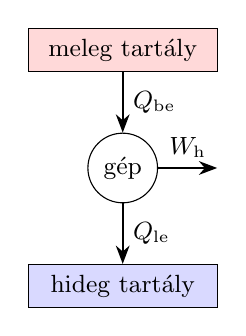
\begin{tikzpicture}[font=\small]
    \node[draw,fill=red!15,minimum width=2.4cm,minimum height=0.55cm] (M) at (0,1.5) {meleg tartály};
    \node[draw,circle,minimum size=0.75cm] (G) at (0,0) {gép};
    \node[draw,fill=blue!15,minimum width=2.4cm,minimum height=0.55cm] (H) at (0,-1.5) {hideg tartály};
    \draw[-{Stealth},thick] (M) -- node[right] {$Q_\text{be}$} (G);
    \draw[-{Stealth},thick] (G) -- node[right] {$Q_\text{le}$} (H);
    \draw[-{Stealth},thick] (G) -- node[above] {$W_\text{h}$} (1.2,0);
  \end{tikzpicture}
\end{minipage}

\newpage
\begin{minipage}[t]{0.70\linewidth}\vspace{0pt}
\begin{enumerate}[start=4]
\item \textbf{Fő feladat.} Az előző órán vizsgált körfolyamat, most \emph{ellenkező
  irányban} körbejárva (figyelj: a $B$ és a $D$ pont felirata is felcserélődött!).
  Egyatomos ideális gáz ($c_V = \tfrac32 R$, $c_p = \tfrac52 R$):
  $A\,(p_0, V_0) \to B\,(2p_0, V_0)$ izochor melegítés,
  $B \to C\,(2p_0, 2V_0)$ izobár tágulás, $C \to D\,(p_0, 2V_0)$ izochor hűtés,
  végül $D \to A$ izobár összenyomás.
  \begin{enumerate}
    \item Fejezd ki az állapotegyenlet segítségével mind a négy pont hőmérsékletét
      $p_0$, $V_0$ és $n$ segítségével!
    \item Számold ki szakaszonként a közölt hőt és a gázon végzett munkát,
      $p_0V_0$ egységekben kifejezve!
    \item Melyik szakaszokon vesz fel hőt a gáz? Mennyi a felvett hő összesen?
    \item Mennyi a hasznos munka? Ellenőrizd két módon: a szakaszonkénti munkák
      összegéből és a diagramról leolvasott területből!
    \item Mekkora a körfolyamat hatásfoka?
    \item Ellenőrzés: mennyi a belső energia megváltozása a teljes körfolyamat alatt?
      Egyezik-e ez a szakaszonként kiszámolt értékek összegével?
  \end{enumerate}
\end{enumerate}
\end{minipage}\hfill
\begin{minipage}[t]{0.27\linewidth}\vspace{0pt}\centering
  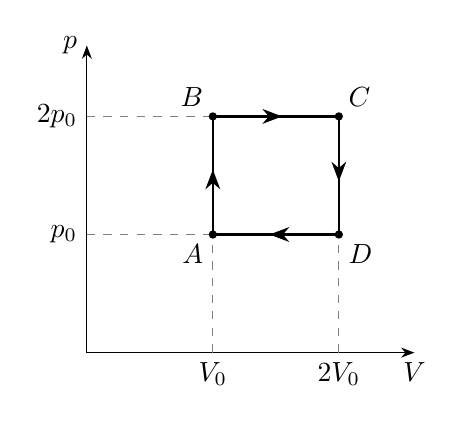
\begin{tikzpicture}[x=1.6cm,y=1.5cm]
    \draw[-{Stealth}] (0,0) -- (2.6,0) node[below] {$V$};
    \draw[-{Stealth}] (0,0) -- (0,2.6) node[left] {$p$};
    \draw[dashed,gray] (1,0) node[below,black] {$V_0$} -- (1,1);
    \draw[dashed,gray] (2,0) node[below,black] {$2V_0$} -- (2,1);
    \draw[dashed,gray] (0,1) node[left,black] {$p_0$} -- (1,1);
    \draw[dashed,gray] (0,2) node[left,black] {$2p_0$} -- (1,2);
    \draw[thick,midarrow] (1,1) -- (1,2);
    \draw[thick,midarrow] (1,2) -- (2,2);
    \draw[thick,midarrow] (2,2) -- (2,1);
    \draw[thick,midarrow] (2,1) -- (1,1);
    \foreach \p/\n/\pos in {{(1,1)}/A/below left, {(1,2)}/B/above left,
                            {(2,2)}/C/above right, {(2,1)}/D/below right}
      \fill \p circle (1.5pt) node[\pos] {$\n$};
  \end{tikzpicture}
\end{minipage}

\vspace{8pt}
\begin{enumerate}[start=5]
\item A 4.~feladat körfolyamatában melyik a legmagasabb és melyik a legalacsonyabb
  hőmérsékletű állapot? Két ilyen hőmérsékletű hőtartály között működő gép hatásfoka
  legfeljebb $1 - T_\text{hideg}/T_\text{meleg}$ lehet. Számold ki ezt a felső korlátot,
  és hasonlítsd össze a 4.~feladatban kapott hatásfokkal! Mit mond ez a mi
  körfolyamatunkról?
\end{enumerate}

\end{document}
